% Created 2018-04-06 Fri 22:50
\documentclass[11pt]{report}
\usepackage[utf8]{inputenc}
\usepackage[T1]{fontenc}
\usepackage{fixltx2e}
\usepackage{graphicx}
\usepackage{longtable}
\usepackage{float}
\usepackage{wrapfig}
\usepackage{rotating}
\usepackage[normalem]{ulem}
\usepackage{amsmath}
\usepackage{textcomp}
\usepackage{marvosym}
\usepackage{wasysym}
\usepackage{amssymb}
\usepackage{hyperref}
\tolerance=1000
\usepackage{minted}
\renewcommand\maketitle{}
\usepackage[margin=0.8in]{geometry}
\usepackage{amssymb,amsmath}
\usepackage{fancyhdr} %For headers and footers
\pagestyle{fancy} %For headers and footers
\fancyfoot[CE,CO]{}
\fancyhead[LE,LO]{}
\usepackage{lastpage} %For getting page x of y
\usepackage{float} %Allows the figures to be positioned and formatted nicely
\restylefloat{figure} %and this command
\usepackage{hyperref}
\hypersetup{urlcolor=blue}
\usepackage{titlesec}
\setcounter{secnumdepth}{4}
\usepackage{minted}
\setminted{frame=single,framesep=10pt}
\rfoot{\thepage\ of \pageref{LastPage}}
\usepackage[parfill]{parskip}
\usepackage{subfig}
\hypersetup{colorlinks=true,linkcolor=black, citecolor=black}
\usepackage{titlesec}
\renewcommand{\bibname}{References}
\usepackage{framed}
\usepackage{etoolbox}
\date{}
\title{\textbf{Modelling the effects of domestication in Wheat through novel computer vision techniques}}
\hypersetup{
  pdfkeywords={},
  pdfsubject={},
  pdfcreator={Emacs 25.3.50.2 (Org mode 8.2.10)}}
\begin{document}

\maketitle
\hyphenpenalty=10000


\titleformat{\chapter}[display]
   {\normalfont\huge\bfseries}{\chaptertitlename\ \thechapter}{20pt}{\Huge}
\titlespacing*{\chapter}{10pt}{10pt}{10pt}


% Redefine the plain page style
\fancypagestyle{plain}{%
  \fancyhf{}%
  \renewcommand{\headrulewidth}{0pt}% Line at the header invisible
  \rfoot{\thepage\ of \pageref{LastPage}}
  \fancyfoot[CE,CO]{}
}

% \patchcmd{\chapter}{\thispagestyle{fancy}}{\thispagestyle{fancy}}{}{}


\thispagestyle{empty}
\renewcommand{\headrulewidth}{0pt}
\begin{center}
  \fontsize{10}{12}
  \selectfont

  \textbf{\huge Modelling the effects of domestication in Wheat through novel computer vision techniques}

  \vspace{0.3in}

  \begin{tabular}[t]{ll}
    Author: & Nathan Hughes (nah26@aber.ac.uk) \\
    Supervisor: & Dr. Wayne Aubrey (waa2@aber.ac.uk) \\
    Degree Scheme &  G401 \hspace*{0.05in}(Computer Science)\\
    \\
    \\
    Date: & \today \\
    Revision: & 0.1\\
    Status: & Draft\\
    \\
  \end{tabular}
  \\
  \vspace{0.1in}
  This report was submitted as partial fulfilment \\of a BSc degree in Computer Science (G401)
\end{center}
\clearpage
\renewcommand{\headrulewidth}{1pt}

\thispagestyle{plain}

\begin{center}
  {\LARGE\bf Declaration of originality}
\end{center}

I confirm that:

\begin{itemize}
\item{This submission is my own work, except where
    clearly indicated.}

\item{I understand that there are severe penalties for Unacceptable Academic Practice, which can lead to loss of marks or even the withholding of a degree.}

\item{I have read the regulations on Unacceptable Academic Practice from the University's Academic Quality and Records Office (AQRO) and the relevant sections of the current Student Handbook of the Department of Computer Science.}

\item{In submitting this work I understand and agree to abide by the University's regulations governing these issues.}
\end{itemize}

\vspace{2em}
Name ............................................................  \\

\vspace{1em}
Date ............................................................ \\

\vspace{1em}
\begin{center}
  {\LARGE\bf Consent to share this work}
\end{center}

By including my name below, I hereby agree to this dissertation being made available to other students and academic staff of the Aberystwyth Computer Science Department.

\vspace{2em}
Name ............................................................  \\

\vspace{1em}
Date ............................................................ \\

\clearpage
\tableofcontents
\listoftables
\listoffigures
\listoflistings
\clearpage


\chapter{Introduction, Analysis and Objectives}
\label{sec-1}

This project aims to answer a biological research question through the use of computer science, whilst also creating a software suite which will enable further studies to be carried out with ease.

Primarily the focus has been on the data science elements of my degree, creating, cleaning and discerning meaning in it.

Additionally, as this is very much multi-disciplinary research, specific terms and definitions have been outlined in the \emph{glossary} (table:\ref{tab:glossary}).

\section{Background}
\label{sec-1-1}

Western society and agriculture has been dominated by the ability to create successful crops for the past 10,000 years \cite{Ozkan2002}. Of these crops Wheat is considered to be one of the most vital and is estimated to contribute to 20\% of the total calories and proteins consumed worldwide, and accounts for roughly 53\% of total harvested area (in China and Central Asia) \cite{Shiferaw2013}.

During domestication, the main traits selected for breeding were most likely plant height and yield. This meant that important non-expressed traits such as disease resistance and drought tolerance were often neglected and lost overtime.

Whilst the choices made for selective breeding were successful, effects are now being felt as it is estimated that as much as a 5\% dip is observed yearly on Wheat production \cite{Shiferaw2013}. This decrease in efficiency is attributed to climate change bringing in more hostile conditions, which these elite and thoroughly domesticated genotypes are unprepared for.

Modern breeding programs have had some success in selecting primitive undomesticated genotypes and using them to breed back in useful alleles which would have been lost during domestication \cite{Charmet2011}.

To create a better understanding of Wheat and in particular how its traits have evolved over time, through domestication, a newly developed method of \textmu{}-CT image analysis \cite{Hughes2017} for crops was used to generate data.

These data were then used to test a number of hypothesis on the effects of domestication in the Wheat genome.

\section{Significance to current research}
\label{sec-1-2}
The biological interest in this area has been expressed in several areas of research \cite{Leigh2013}, it is proposed that the key to unlocking diversity in the Wheat genus lies in these ancestor, undomesticated species \cite{Cockram2007}.

This research has the potential to be useful in several areas including: crop breeding; disease resistance; environmental stress.

The individual images in figure:\ref{fig:phylo} show, at a glance, the diversity and also the difference in the wild and cultivated (domesticated)
species. This work allows for these differences to be quantified and evaluated into useful metrics for answering research based questions.

\begin{figure}[htb]
\centering
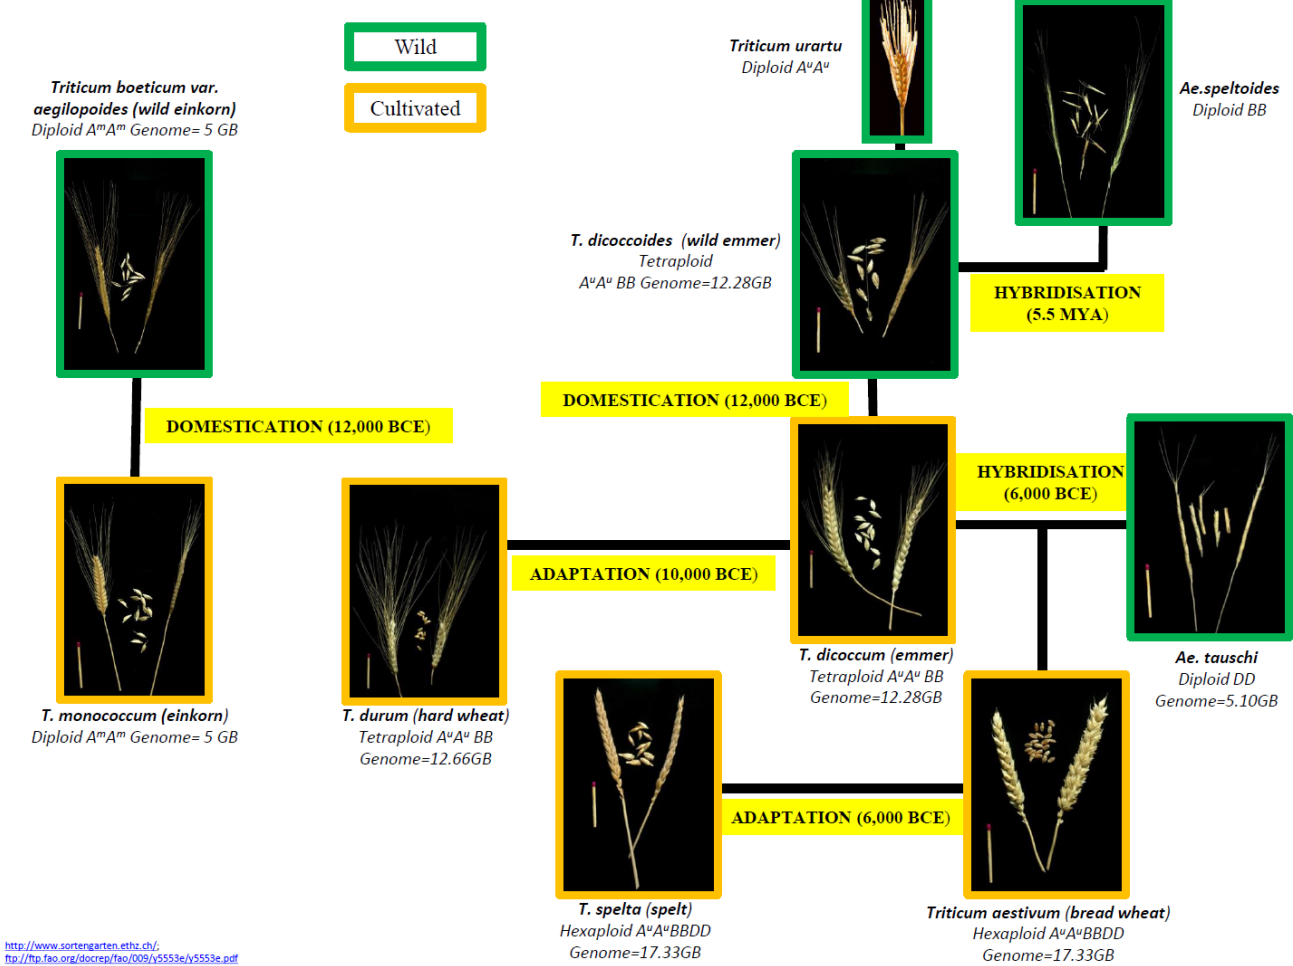
\includegraphics[width=17cm]{./images/philotree.png}
\caption{\label{fig:phylo}Phylogeny of wheat genotypes (Provided by Dr. Hugo Oliveira)}
\end{figure}

\section{Hypothesis}
\label{sec-1-3}

To provide a full spectrum of analysis the null-hypothesis of this work is presented as investigating if there are morphometric differences in the seeds of several wheat varieties outlined in figure:\ref{fig:phylo}.

The comparison pairs are as follows:

\begin{enumerate}
\item Wild Einkorn and Domesticated Einkorn
\item Wild Emmer and Domesticated Emmer
\item Bread Wheat and Spelta Wheat
\item Domesticated Emmer and Durum
\item Wild Einkorn and Wild Emmer
\end{enumerate}

\section{Aim and Objectives}
\label{sec-1-4}

The overarching aim of this project has been to create several pieces of software which aid in answering the biologically significant questions outlinned. As well as to prove/disprove the hypothesis stated.

The software created is robust in order to duplicate results and is flexible as to allow for further studies to be carried out and to use the same method.

Novel additions have been made to existing image analysis libraries in order to make them more flexible for this project.

Furthermore, the library written allows for easy data organisation and automation of otherwise difficult tasks such as concatenating data from multiple sources and graphing of information. Full documentation and integrated testing allows for a suite of tools which can be built upon in future and reduce the amount of effort required for similar studies to be carried out and analysed.

\section{Deliverables}
\label{sec-1-5}

This project provides three final deliveribles:

\begin{enumerate}
\item A flexible software suite written in \emph{Python} that provides a standardised method for analysing and interpreting \textmu{}-CT data output.
\item A Graphical User Interface (GUI) which offers a point and click method for data gathering, graphing and manipulating \textmu{}-CT data, using the library from deliverable 1 as a backend.
\item Answers to the proposed questions (hypothesis), the \emph{Results} and \emph{Discussion} sections of this report provides this.
\end{enumerate}

\chapter{Method Design}
\label{sec-2}

\section{Improvements to 3D imaging software}
\label{sec-2-1}
\subsection{{\bfseries\sffamily TODO} PACIFY New Watershed Algorithm}
\label{sec-2-1-1}

In order to solve the problem of misidentified and joint seeds, from the primitive collection,
I implemented a \emph{quasi-euclidean} distance transform into the analysis pipeline \cite{Hughes2017}. This provided much better results than the previous
\emph{chessboard} transform which had been successful on more uniform data.

\subsubsection{Quasi-Euclidean algorithm}
\label{sec-2-1-1-1}

This algorithm measures the total euclidean distance along a set of horizontal, vertical and diagonal
line segments \cite{Pfaltz1966}.

\begin{equation}
\label{eqn:qe}
\left | x_1 - x_2 \right | + (\sqrt{2}-1), \left | x_1 - x_2 \right | >\left | y_1 - y_2 \right | (\sqrt{2}-1) \left | x_1 - x_2 \right | ,\textup{otherwise}
\end{equation}


In order to apply this to a 3D space Kleinberg's method is used  \cite{Kleinberg1997}. This allows for nearest neighbour pixels to be sorted by $k$-dimensional trees
and enabling fast distance transforms via Rosenfeld and Pfaltz's \emph{quasi-euclidean} method stated in equation:\ref{eqn:qe}.


\section{Testing of Software}
\label{sec-2-2}

\chapter{Software Design, Testing and Implementation}
\label{sec-3}

\section{Software Development Methodology}
\label{sec-3-1}

\section{Data Pipeline}
\label{sec-3-2}

\begin{center}
\begin{figure}[htb]
\centering
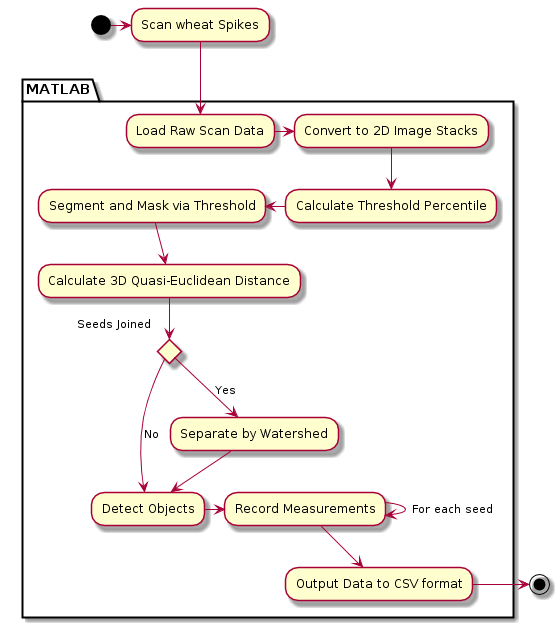
\includegraphics[width=10cm]{./images/matlab.png}
\caption{\label{fig:matlab}Image Processing Pipeline}
\end{figure}
\end{center}


\begin{center}
\begin{figure}[htb]
\centering
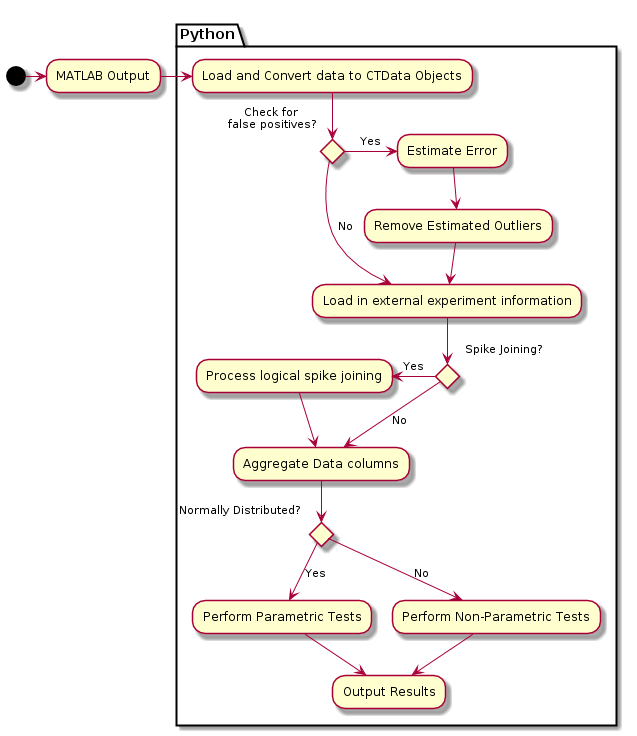
\includegraphics[width=10cm]{./images/pipeline.png}
\caption{\label{fig:pipeline}Data Pipeline and Information Flow}
\end{figure}
\end{center}

\chapter{Results}
\label{sec-4}

\section{Improved accuracy of imaging software}
\label{sec-4-1}

\subsection{Effect of enhanced watershedding algorithm}
\label{sec-4-1-1}
\begin{center}
\begin{figure}[htb]
\centering
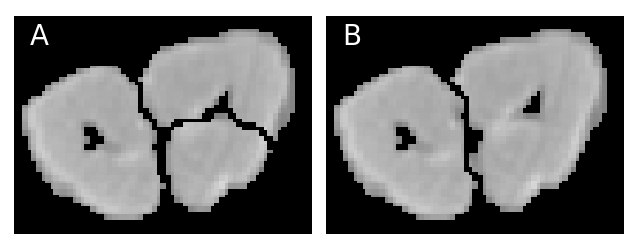
\includegraphics[width=10cm]{./images/chess_quasi.png}
\caption{\label{fig:qe}\emph{A} showing the chessboard method, \emph{B} improved quasi-euclidean method}
\end{figure}
\end{center}

\chapter{Discussion}
\label{sec-5}
\chapter{Critical Evaluation}
\label{sec-6}
\section{Organisational Methods}
\label{sec-6-1}
\section{Relevance to Degree}
\label{sec-6-2}
\section{Time Management}
\label{sec-6-3}
\section{Collaborative Work}
\label{sec-6-4}
\section{Other Issues}
\label{sec-6-5}



\chapter{Appendix}
\label{sec-7}
\section{\emph{Software Packages Used}}
\label{sec-7-1}

\subsection{Libraries}
\label{sec-7-1-1}
\begin{table}[htb]
\caption{\label{tab:software}Software libraries used}
\centering
\begin{tabular}{|l|l|l|}
\hline
MATLAB Image Processing Toolbox & Numpy & Matplotlib\\
\hline
Seaborn & Scipy & Sklearn\\
\hline
Statsmodels & Pymc3 & Xlrd\\
\hline
PyQt5 &  & \\
\hline
\end{tabular}
\end{table}

\subsection{Tools}
\label{sec-7-1-2}
\begin{table}[htb]
\caption{\label{tab:softwareused}Software tools used}
\centering
\begin{tabular}{|l|l|l|}
\hline
MATLAB & Python Debugger (PDB) & IPython\\
\hline
Emacs & git & org-mode\\
\hline
Tomviz & ImageJ & \\
\hline
\end{tabular}
\end{table}

\section{\emph{Glossary}}
\label{sec-7-2}
\begin{table}[htb]
\caption{\label{tab:glossary}Dictionary for Terms and acronyms}
\centering
\begin{tabular}{|l|l|}
\hline
\textbf{Term} & \textbf{Definition}\\
\hline
\textmu{}-CT & Micro Computed Tomography\\
\hline
Genotype & A genetically distinct individual or group\\
\hline
Phenotype & A physical/measurable trait\\
\hline
Alleles & A variant of a gene\\
\hline
Genus & \\
\hline
Genome & \\
\hline
Morphometric & \\
\hline
GUI & Graphical User Interface\\
\hline
\end{tabular}
\end{table}


\section{\emph{Code Segments and Examples}}
\label{sec-7-3}
\subsection{MATLAB Watershedding}
\label{sec-7-3-1}


\begin{listing}[H]
\begin{minted}[]{octave}
function [W] = watershedSplit3D(A)
  % Takes image stack A and splits it into stack W
  % Convert to BW
  bw = logical(A);
  % Create variable for opening and closing
  se = strel('disk', 5);
  % Minimise object missshapen-ness
  bw = imerode(bw, se);
  bw = imdilate(bw, se);
  % Fill in any left over holes
  bw = imfill(bw,4,'holes');
  % Use chessboard for distance calculation for more refined splitting
  chessboard = -bwdist(~bw, 'quasi-euclidean');
  % Modify the intensity of our bwdist to produce chessboard2
  mask = imextendedmin(chessboard, 2);
  chessboard2 = imimposemin(chessboard, mask);
  % Calculate watershed based on the modified chessboard
  Ld2 = watershed(chessboard2);
  % Take original image and add on the lines calculated for splitting
  W = A;
  W(Ld2 == 0) = 0;
end
\end{minted}
\caption{\label{lst:ws}MATLAB Watershedding function}
\end{listing}

\clearpage
\addcontentsline{toc}{Chapter}{References}
\bibliography{library}
\bibliographystyle{IEEEannotU}
% Emacs 25.3.50.2 (Org mode 8.2.10)
\end{document}
